\chapter{Lessons from Optimizing Adaptive Mesh Codes}
\label{chap:amr}
\minitoc

\section{Motivation: Computational Efficiency in AMR Codes}

Adaptive Mesh Refinement (AMR)~\cite{Dubey2014:Survey,Grete2023:Parthenon,Zhang2021:AMReX} is a
widely used technique for efficiently simulating physical systems that exhibit large variations in
spatial or temporal scales, such as astrophysical phenomena, fluid dynamics, and climate modeling.
AMR codes dynamically refine and coarsen the computational grid to concentrate resources in regions
of interest, resulting in highly irregular and rapidly evolving mesh structures.
This approach enables fine-grained resolution where needed, but creates significant computational
challenges: the workload becomes highly imbalanced, dependencies between tasks grow complex, and
the dynamic nature of the mesh makes it difficult to achieve efficient parallel execution and
balanced load across compute
resources~\cite{Klenk2017:OverviewMPICharacteristics,Dubey2014:Survey,Burst2008:ALPS}.

Our goal was to develop placement policies that leveraged runtime telemetry to improve placement
and efficiency.
Access to our research cluster enabled us to experiment with fine-grained telemetry and placement
under full-stack administrative control, providing the ability to analyze and intervene at all
levels of the software and hardware stack.

\section{Challenges of Telemetry-Driven Placement}

Developing telemetry-driven placement policies in AMR codes exposed several
key challenges:

\begin{itemize}
  \item \textbf{Establishing measurement fidelity.}
        Initial telemetry was often unreliable and did not match intuition (\cref{fig:amr-tele}).
        Only by using full-stack access and low-level debugging could we identify and correct sources of
        error across hardware, drivers, MPI, and the application.

  \item \textbf{Scaling analysis for high-volume telemetry.}
        Analyzing per-rank, per-timestep telemetry required moving beyond standard profiling and tracing
        tools to query-driven workflows that could surface root causes from massive data.

  \item \textbf{Low-overhead, effective placement.}
        Even with reliable telemetry, incorporating it into placement imposed strict timing constraints and
        required new algorithms to balance objectives like load and locality in dynamic, NP-hard settings.
\end{itemize}

\section{Contribution 1: A Diagnostic Workflow}

The process of developing placement policies required understanding what our telemetry was
capturing.
Initially, our telemetry showed no correlation between expected workload drivers and observed
performance (Figure~\ref{fig:amr-tele-reg}).
Deeper investigation revealed cross-stack artifacts: fail-slow hardware, system tuning issues, and
fabric-level problems that had to be systematically mitigated (\cref{fig:amr-tele-comm}).
Only after this full-stack debugging and tuning process could we obtain reliable telemetry that
correlated with expected application behavior.

While our full-stack access enabled these investigations, we found identifying and isolating these
transient artifacts to be difficult.
We initially used standard profiling and tracing tools~\cite{Shend2006:TAU}, but found the behavior
of our applications to necessitate structured and targeted telemetry collection for analytics.
Profiling often obscured visibility into transient artifacts, while tracing resulted in large
volumes of analytically intractable data.
We organically evolved a workflow for targeted collection of queryable telemetry, starting from CSV
exports analyzed with pandas~\cite{:Pandas}, and culminating in
ClickHouse~\cite{Schul2024:ClickHouse} and SQL queries.
This custom approach enabled correlation of performance data across ranks and system layers,
allowing us to isolate the true sources of performance anomalies.
% This custom approach enabled correlation of performance data across ranks and system layers,
% allowing us to isolate the true sources of performance deviation.

% \section{Motivation: The Problem of Load Imbalance in AMR}

% Adaptive Mesh Refinement (AMR) codes are essential for efficiently simulating physical phenomena
% with large variations in spatial or temporal scales. These applications dynamically refine a
% computational grid in regions of interest, creating a highly irregular and evolving workload. The
% process of assigning these grid blocks to parallel workers is known as placement. A naive
% placement can lead to significant load imbalance, where some workers have far more computation
% than others, causing them to become stragglers that delay the entire application at
% synchronization points.

% The initial goal of this work was to mitigate this widely-assumed problem of algorithmic load
% imbalance. We sought to create a telemetry-driven placement policy that would use fine-grained
% runtime information to create more balanced work assignments for parallel workers, thereby
% improving overall application efficiency.

% \section{The Diagnostic Journey: Uncovering the Real Problem}

% \subsection{The Unreliability of Raw Telemetry}

\begin{figure}[h]
  \begin{subfigure}{0.64\textwidth}
    \centering
    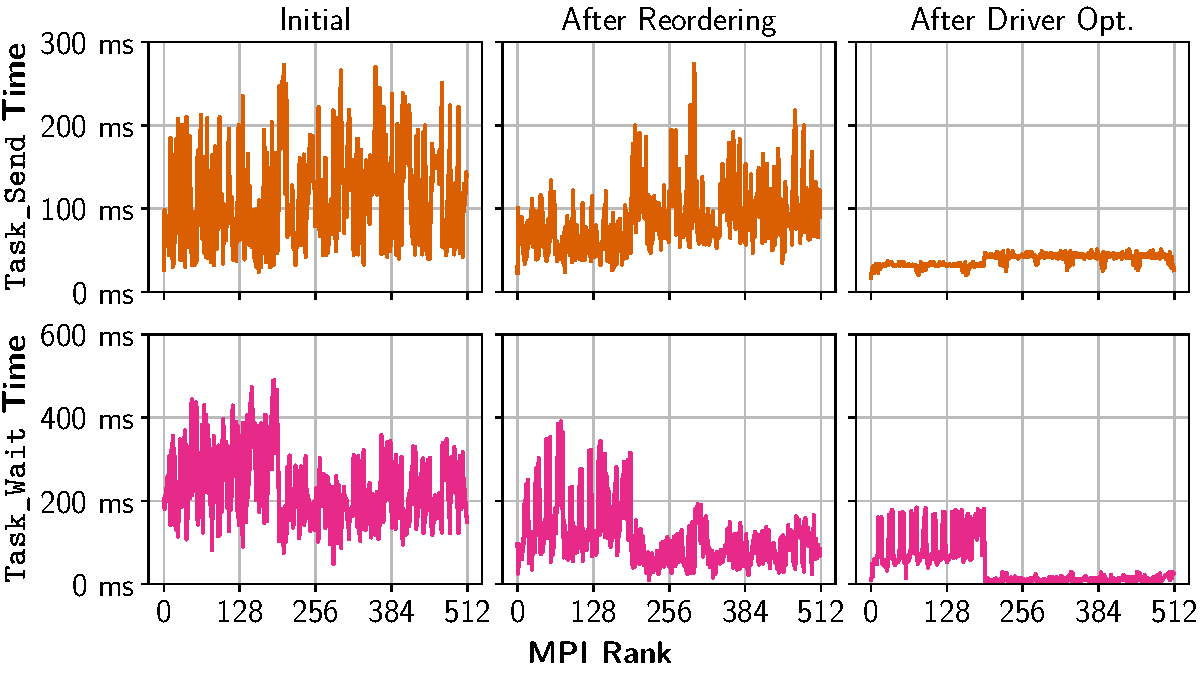
\includegraphics[
      width=\textwidth,trim=0cm 0cm 0cm 0cm,clip
    ]{data/figs/amr_lesson_ordering_v5.pdf}
    \caption{Rank-wise AMR telemetry, before and after tuning}
    \label{fig:amr-tele-comm}
  \end{subfigure}
  \begin{subfigure}{0.36\textwidth}
    \centering
    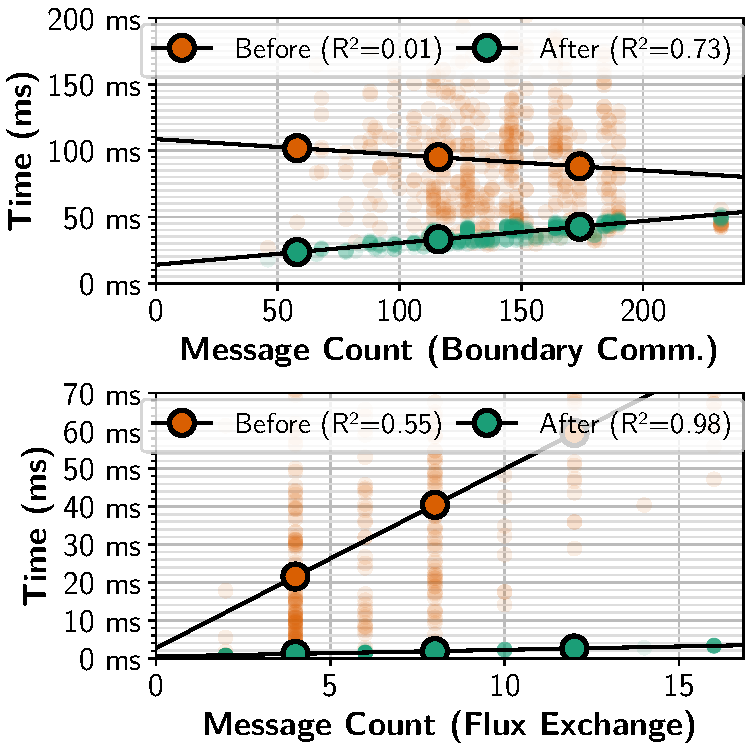
\includegraphics[
      width=\textwidth,trim=0cm 0cm 0cm 0cm,clip
    ]{data/figs/amr_msgcnt_regr_vert.pdf}
    \caption{AMR telemetry regression analysis}
    \label{fig:amr-tele-reg}
  \end{subfigure}
  \caption{
    (Left) Fine-grained per-rank telemetry from communication functions showing significant variability,
    that progressively reduces with tuning.
    (Right) Regression analysis of communication telemetry showing poor initial correlation with work,
    that improves significantly with tuning.
  }
  \label{fig:amr-tele}
\end{figure}

% Our initial efforts to build a model from performance telemetry failed. We observed poor and
% inconsistent correlation between expected workload drivers, such as message counts for a
% communication phase, and the observed performance. This indicated that other factors were
% influencing runtime, forcing us to embark on a deep, cross-stack investigation into the sources of
% this unpredictable variability.

% \subsection{An Evolving Analysis Workflow} This diagnostic process revealed the limitations of the
% standard performance analysis workflow. Initial analysis with profiling tools provided only
% coarse-grained aggregates that obscured transient effects. Examining detailed traces proved to be
% impractical due to the sheer volume of data and the lack of queryable interfaces.

% To make progress, our analysis workflow evolved organically. We moved from standard tools to
% instrumenting the code to emit custom, structured logs. As the scale of this data grew, we
% eventually built a pipeline to ingest it into a relational analytics database. This ad-hoc system
% provided the query-driven, interactive capability necessary to correlate events across ranks and
% system layers, allowing us to isolate the true sources of performance deviation.

% \subsection{Finding: Algorithmic Imbalance vs. System Noise} The key insight from this diagnostic
% journey is that in a complex parallel system, performance variability from different sources can
% be easily conflated. Without the ability to perform fine-grained, query-driven analysis, it is
% impossible to distinguish between true algorithmic load imbalance and performance bottlenecks
% originating from the underlying system. The diagnostic process revealed that many performance
% anomalies manifesting as load imbalance were in fact symptoms of system noise, including hardware
% fail-slow behavior and network driver contention.

\section{Contribution 2: The CPLX Placement Policy}
With reliable telemetry established, we turned to the challenge of developing more effective
placement policies.
Placement strategies for AMR codes have traditionally prioritized maximal preservation of
communication locality
~\cite{Warre1993:ParallelHashedOctTree,Sasid2015:GeneralSpacefillingCurve,Bhate2011:ApplyingGraphPartitioning,Catal2007:Zoltan,Lasal2013:parMETIS},
using tools like \emph{Space-Filling Curves}~\cite{Burst2011:p4est} (SFCs) to co-locate spatially
adjacent grid blocks.
However, we recognized that for computationally variable workloads, an exclusive focus on locality
is fundamentally at odds with achieving good load balance.
This led us to reframe placement as not about maximizing a single objective, but about explicitly
managing the trade-off between communication and computation to minimize overall runtime.

To navigate this trade-off, we developed CPLX, a policy that provides predictable control over
locality and load balance through a single tunable parameter, $\mathsf{X}$.
CPLX operates as a hybrid of two underlying policies: a locality-preserving dynamic programming
approach (CDP) developed by us and the load-balancing-focused \emph{Longest Processing Time} (LPT)
heuristic~\cite{Graha1969:LPT}.
The algorithm first computes a locality-aware placement using CDP.
It then identifies the $\mathsf{X}\%$ most imbalanced ranks (both overloaded and underloaded) and
rebalances \emph{only} their assigned work using LPT, leaving the rest of the placement untouched.
This mechanism allows CPLX to smoothly interpolate between a fully locality-preserving policy
($\mathsf{X}=0$) and a pure load-balancing policy ($\mathsf{X}=100$), enabling empirical tuning of
the trade-off.

% CPLX provides predictable control over the tradeoff between locality and load balance through a
% single tunable parameter $\mathsf{X}$. At $\mathsf{X}=0$, CPLX is locality maximizing; at
% $\mathsf{X}=100$, CPLX is pure computational load balance. CPLX is a hybrid of two policies: CDP
% (a locality-maximizing policy based on \emph{dynamic programming} developed by us) and LPT
% (\emph{Longest Processing Time}~\cite{Graha1969:LPT}). The algorithm computes an initial placement
% using CDP, then examines allocated load among ranks and only rebalances $\mathsf{X}\%$ of the most
% overloaded and underloaded ranks, preserving locality for well-balanced portions.

\begin{figure}[h]
  \centering
  
\includegraphics[
    width=\textwidth,trim=0.2cm 0cm 0.1cm 0cm,clip
  ]{data/figs/amr_blastwave_runtime_wide.pdf}
  \caption{End-to-end AMR code runtime as a function of policy at four scales (512--4096 ranks), classified
    into four phases.
    CPLX achieves up to 21.6\% runtime reduction over already-optimized baselines.
    Total runtime follows a U-shaped curve as X increases, with best performance at intermediate
    values, from balancing the constituent tradeoffs.
    Impact of CPLX increases with scale.
  }
  \label{fig:amr-eval-rt}
\end{figure}

\section{Key Results}


We evaluated our placement policies on our in-house research cluster using the
Phoebus~\cite{Barke2024:Phoebus} code built on the Parthenon AMR
framework~\cite{Grete2023:Parthenon}, at scales ranging from 512 to 4096 ranks.
We chose the Sedov blast wave~\cite{Sedov1959:SimilarityDimensionalMethods} problem as our
workload, as its dynamic refinement patterns make it a challenging test case for placement
policies.
All comparisons are against the tuned baseline using standard SFC-based placement.

As shown in Figure~\ref{fig:amr-eval-rt}, CPLX achieves up to a 21.6\% runtime reduction over the
optimized baseline.
Overall performance follows a U-shaped curve as $\mathsf{X}$ is varied, with the best results
achieved at intermediate values.
At $\mathsf{X}=0$, CPLX is locality maximizing at the expense of of suboptimal load balance, while
at $\mathsf{X}=100$, CPLX completely disregards locality to maximize load-balance.
Minimum runtime is achieved at intermediate $\mathsf{X}$ values by balancing the constituent
trade-offs.
The impact of CPLX and managing the trade-off both increase with scale.

\section{Lessons}

Elevated synchronization time in AMR codes is commonly ascribed to algorithmic load imbalance.
While execution variability is a known
issue~\cite{Petri2003:Missing,Hoefl2010:Noise,Gunaw2018:FailSlow,Gangi2024:RDMA,Acun2016:Variation,Acun2016:Mitigating,Yildi2016:IONoise},
it is often overlooked in performance analyses, which are typically conducted offline and
disconnected from runtime context~\cite{Klenk2017:OverviewMPICharacteristics}.
Our work shows that accurate diagnosis requires holistic, in situ performance analysis to isolate
the true sources of variability.
We find that algorithmic techniques can improve placement, but they also expose tunable
tradeoffs---such as load balance versus communication locality---whose optimal configuration also
benefits from real-time visibility into application behavior.
Our organically evolved pipeline demonstrates the value of structured, queryable telemetry, and
motivates the realization of real-time observability capabilities tailored to the needs of
tightly-coupled parallel applications.

% Our structured telemetry pipeline offers a path beyond ad hoc tooling---toward queryable,
% programmable observability that supports principled diagnosis and tuning. The primary challenge
% was not algorithmic optimization, but understanding performance behavior within the constraints of
% specific hardware and software stacks. This underscores the need for real-time visibility into
% application performance. Our structured telemetry pipeline offers a path beyond ad hoc
% tooling—toward queryable, programmable observability that supports principled diagnosis and tuning

% Elevated synchronization time in AMR codes is commonly ascribed to algorithmic load imbalance in
% performance analyses. While execution variability is a known problem, it is typically not factored
% into performance analyses, which are often conducted separately from data collection. Our work
% demonstrates the importance of carrying out a holistic performance analysis in-situ to identify
% and isolate the true sources of performance variability. This requires real-time visibility into
% application performance for effective diagnosis and tuning. The biggest bottleneck was
% understanding performance rather than algorithmic optimization, as performance characteristics are
% inherently idiosyncratic to specific hardware and software stacks. Our structured telemetry
% pipeline demonstrates the path forward from ad-hoc tools to queryable, programmable observability.

\newpage